\section{Notation}
\label{app:notation}

\begin{table}[!htb]
  \centering
  \caption{\textbf{Notation.}}
  \label{tab:notation}
  \small
  \begin{tabular}{@{}ll@{\qquad}ll@{}}
    \toprule
    \textbf{Symbol} & \textbf{Meaning} & \textbf{Symbol} & \textbf{Meaning} \\
    \midrule
    $F_i$ & frames in the stream of item $i$ & $\lambda$ & commit threshold on $s_i$ \\
    $V$ & vocabulary size of the stream & $s_i$ & commit score of item $i$ (\cref{sec:crc}) \\
    $K$ & size of the candidate list ($K = 10$) & $n$ & number of calibration items \\
    $k$ & number of offered candidates & $T$ & number of items in an online sequence \\
    $\tau_f$, $\tau_s$ & frame and sentence temperatures & $\eta$, $\gamma$ & step sizes of the online controllers \\
    $c_i$, $f_i$ & commit loss, non-commit loss & $\alpha$, $\delta$ & target risk, LTT failure probability \\
    \bottomrule
  \end{tabular}
\end{table}

\section{User model parameters}
\label{app:user}

\Cref{tab:user} lists the parameters of the simulated gaze-typing user (word model: the user fixes single words). Only the fallback typing speed and the per-slot scan-and-select time are matched to measurements of one eye-gaze user with ALS \citep{cai2024gaze}; all other values are assumptions. The baseline ``gaze typing only'' uses the fallback speed alone.

\begin{table}[!htb]
  \centering
  \caption{\textbf{Simulated-user parameters.}}
  \label{tab:user}
  \small
  \begin{adjustbox}{max width=\linewidth}\begin{tabular}{@{}lll@{}}
    \toprule
    \textbf{Parameter} & \textbf{Value} & \textbf{Basis} \\
    \midrule
    Fallback (gaze keyboard) speed & 20 characters/min & measured, eye-gaze user LP1 \citep{cai2024gaze} \\
    Scan and select one of $k$ word alternatives & $1.0 + 1.0\log_2(k+1) + 1.5$\,s (4.5\,s for $k = 3$) & sum matched to 4.7\,s \citep{cai2024gaze} \\
    Select one of $k$ offered sentences & $1.0 + 0.5\log_2(k+1)$\,s & assumption \\
    Reading time & 0.3\,s per word, 0.5\,s per candidate & assumption \\
    Navigate to and delete a wrong word & 3.0\,s (2 selections) & assumption \\
    Miss probability of a wrong, unmarked word (commit, \act{offer\_words}) & 0.05 & assumption (no measurement) \\
    Errors in offered candidates & always seen & assumption \\
    Full retype overhead & 1.5\,s; chosen when cheaper than fixing words & assumption (rational user) \\
    Abstain overhead & 0.5\,s, then fallback typing & assumption \\
    Neural input speed, MEG / B2T '25 / sEMG & 152 / 159.3 / 75.8 characters/min & device setting \\
    \bottomrule
  \end{tabular}\end{adjustbox}
\end{table}

\section{Per-device settings}
\label{app:settings}

\Cref{tab:settings} lists the parameters that the shared implementation fitted or used per device. The policy grid and all decoder settings are in the experiment configurations in the repository.

\begin{table}[!htb]
  \centering
  \caption{\textbf{Per-device settings of the shared trust-layer implementation.} Fitted on each device's fit data (MEG: validation set). $\tau_s = 20.0$ is the upper end of the search interval. Max.\ guard risk: largest guard risk that still allows a commit.}
  \label{tab:settings}
  \small
  \begin{adjustbox}{max width=\linewidth}\begin{tabular}{@{}lllll@{}}
    \toprule
    & \textbf{MEG} & \textbf{B2T '25, ours} & \textbf{B2T '25, published gate} & \textbf{sEMG (cal.\ / x-sess.\ / x-subj.)} \\
    \midrule
    Frame temperature $\tau_f$ & 3.30 & 3.78 & 3.78 & 1.25 / 1.78 / 2.17 \\
    Sentence temperature $\tau_s$ & 20.0 & 4.56 & 1.72 & 2.42 / 5.42 / 20.0 \\
    LM weight (beam) & 0.5 & 1.0 (word LM; edit penalty 12, word bonus 3) & as ours & 1.0 / 1.0 / 1.5 \\
    Candidate list $K$ & 10 & 10 & published sentence + our 10 (bonus +2.0) & 10 \\
    Plug-in commit threshold & 0.5 & 0.5 & 0.7 & 0.7 / 0.3 / 0.3 \\
    Max.\ guard risk for commit & 0.3 & 0.5 & 0.5 & 1.0 / 1.0 / 0.1 \\
    Offer size $k$ & 1 & 2 & 1 & 2 / 2 / 1 \\
    Fallback after offer & offer & offer & offer & offer \\
    Guard & \multicolumn{4}{l}{low-evidence threshold 0.5; consistency over the top 5; risk $=\max$(low evidence, 1 $-$ consistency), weights 1} \\
    Adapter (lines of Python) & 148 & 412 & 412 & 568 \\
    \bottomrule
  \end{tabular}\end{adjustbox}
\end{table}

\section{MEG decoder, leakage checks and sensitivity}
\label{app:meg}

The asynchronous MEG decoder is a convolutional front end (320 channels) followed by 4 Conformer layers of width 256 \citep{gulati2020conformer}, trained with CTC \citep{graves2006ctc} and a keystroke auxiliary loss that uses key times as training labels (key pretraining, then CTC training on all 80 recording blocks). At inference, the forward pass takes the MEG segment, its length and the participant index; it has no key input. \Cref{tab:async} compares the inference inputs with the published asynchronous decoder.

\begin{table}[!htb]
  \centering
  \caption{\textbf{Asynchronous setting: our decoder vs Brain2Qwerty v2.}}
  \label{tab:async}
  \small
  \begin{tabular}{@{}lll@{}}
    \toprule
    \textbf{Input at inference} & \textbf{Ours} & \textbf{v2 async \citep{zhang2026brain2qwertyv2}} \\
    \midrule
    MEG of the sentence segment & yes & yes \\
    Segment start & first key $-$ 0.4\,s & first key $-$ 400\,ms \\
    Segment end & last key press + 0.5\,s & last key release + 400--500\,ms \\
    Per-key times or key count & no & no \\
    Participant index & yes & yes \\
    Key times as training labels & yes (auxiliary loss) & no \\
    \bottomrule
  \end{tabular}
\end{table}

\paragraph{Leakage checks.} The split is by a hash of the sentence text, and no test sentence occurs in the LM training text. A test sentence is ``close'' if a training sentence is within CER 0.25; 6 of the 17 test sentences are close. Without them, the CER was 0.519 (greedy) and 0.492 (beam).

\paragraph{Synchronous control decoder.} A synchronous decoder with oracle key times (greedy CER 0.508, beam + LM 0.447; harness top-1 CER 0.451) gave the same trust results as the asynchronous decoder: always commit 2.714, trust 3.229 and gaze typing 3.155 \ewpm{}, trust minus gaze \ci{-0.02}{+0.18} over sentences and \ci{-0.07}{+0.26} two-way. Over trials, this difference excluded 0 (\ci{+0.03}{+0.12}): trial-level intervals make the MEG result look like a gain, and sentence-level intervals do not. Both decoders take the sentence bounds from the keyboard log, so neither is a free-running decoder. \todo{R1: k-fold over sentence hashes to increase the number of unique MEG test sentences.}

\paragraph{User-model sensitivity on MEG.} \Cref{tab:megsens} refits the policy under each user-model variant (asynchronous decoder). The trust layer equals always offering in every variant. The advantage over always commit depends on the miss probability, and the comparison with gaze typing reverses with a faster fallback or slower selection. \todo{R1: the same grid on B2T '25 and sEMG, with the policy ranking and a misspecified-user evaluation.}

\begin{table}[!htb]
  \centering
  \caption{\textbf{User-model sensitivity, MEG (asynchronous decoder; policy refitted per variant).} \ewpm{}; CIs over the 17 unique sentences and over the 19 participants.}
  \label{tab:megsens}
  \small
  \begin{adjustbox}{max width=\linewidth}\begin{tabular}{@{}lllllll@{}}
    \toprule
    \textbf{Variant} & \textbf{Always commit} & \textbf{Trust} & \textbf{Gaze only} & \textbf{Trust $-$ gaze [sent.]} & \textbf{\{part.\}} \\
    \midrule
    Main (miss 0.05, fallback 20 cpm) & 2.58 & 3.20 & 3.15 & \ci{-0.04}{+0.15} & \{$-$0.07, +0.22\} \\
    Fallback 40 characters/min & 4.31 & 5.15 & 6.31 & \ci{-1.29}{-1.01} & \{$-$1.31, $-$0.95\} \\
    Miss probability 0 & 3.24 & 3.20 & 3.15 & \ci{-0.04}{+0.15} & \{$-$0.08, +0.22\} \\
    Miss probability 0.2 & 1.24 & 3.20 & 3.15 & \ci{-0.04}{+0.15} & \{$-$0.08, +0.22\} \\
    Selection, scan and navigation $\times 2$ & 2.54 & 3.00 & 3.15 & \ci{-0.23}{-0.08} & \{$-$0.26, $-$0.02\} \\
    No full retype & 2.54 & 3.18 & 3.15 & \ci{-0.06}{+0.13} & \{$-$0.10, +0.21\} \\
    \bottomrule
  \end{tabular}\end{adjustbox}
\end{table}

\section{Format details and audit log}
\label{app:format}

\paragraph{Serialisations and conformance.} The reference serialisations of \nts{} are an NPZ file and a JSON Lines streaming form. A conformance suite runs 60 checks, each tied to a specification clause, and reports one of three cumulative levels: \emph{core} (a consumer must accept the stream), \emph{trust-ready} (modality, causality, calibration state and language are declared) and \emph{provenance} (stream id, decoder name, version and weights hash). It ships 52 golden test vectors (32 NPZ, 20 JSON Lines); the reference consumer passes 52 of 52. On synthetic inputs, our MEG and sEMG adapters reach the provenance level and the intracortical adapter reaches trust-ready, because the published online decoder has no weights file to hash. Writing the suite found five bugs in our own producers and ten ambiguities in the specification text, now listed as open questions.

\paragraph{Audit log.} Each decision can be appended to a JSON Lines log. Context entries are content-addressed (their id is the SHA-256 of the context) and hold the adapter, decoder (name, version, weights hash, training data and licence), LM, calibration (temperatures, risk-control method, $\alpha$, $\delta$, threshold, $n$) and policy versions; decision entries hold the action, scores, a hash of the stream and its frame range; correction entries link to the decision they correct. Each entry stores the hash of the previous entry and its own SHA-256 over the canonical JSON, so any edit, deletion or reordering breaks the chain; a separately stored head anchor detects truncation. The log stores no raw signals (numeric arrays longer than 64 values are rejected), stores text as a keyed hash by default, and pseudonymises subject and session ids. It is tamper-evident, not tamper-proof: there is no signature in v0.

\paragraph{Replay.} We replayed the Brain-to-Text '25 test half (816 trials) with the log attached, for the plug-in gate and a CRC gate. The log held 1,723 entries and passed verification. It recorded the same wrong commits as the harness: 48 of 48 (plug-in) and 39 of 39 (CRC), of which 2 and 1 were silent. This is a consistency check of the replay: the corrections come from the known cue sentences, and in live use silent errors would be missing from the log. Every tampering case we tried was detected: editing an entry, editing with re-hashing, deleting, reordering, and cutting the tail (with the head anchor). The cost was about 0.1\,ms and about 1.1\,kB per decision. \Cref{fig:audit} shows one entry of the audit report.

\begin{figure}[!htb]
  \centering
  \fbox{\begin{minipage}{0.94\linewidth}\footnotesize\raggedright
  \textbf{Wrong commit} \texttt{dec-000041-ed60b4bd} (entry 44, hash \texttt{8cf2c6c67053b185...})\\
  Committed: ``who you never expect to when''\\
  Correction (known cue sentence, hash-linked): ``who you never expect to win''; 2 character edits, 1 word edit\\
  Scores: $\hat p_{\mathrm{top1}}$ 0.5814, set size 3, guard risk 0.2857; reason: $\hat p_{\mathrm{top1}} \ge 0.50$\\
  Input: stream \texttt{1b4b60e8e4950710...}, frames [0, 335], item \texttt{b2t25-test-trial-196}\\
  Decoder: published online RNN + our phoneme-to-word decoder; LM: Tatoeba character 6-gram + word unigram + CMUdict; adapter \texttt{fidetype.adapters.b2t25}\\
  Calibration \texttt{cal-692fb52a73417552}: $\tau_f$ 3.7809, $\tau_s$ 4.5551, fit set: first half of each day (812 trials)\\
  Policy \texttt{pol-2eaa4ff51919527a}: commit threshold 0.5, maximum guard risk 0.5, offer size 2
  \end{minipage}}
  \caption{\textbf{One entry of the audit report} (B2T '25 replay, plug-in gate; public CC0 cue sentence). Each wrong commit is traced to the exact stream segment and to the decoder, LM, calibration and policy versions that produced it. Hashes are shortened.}
  \label{fig:audit}
\end{figure}

\section{Online re-calibration methods}
\label{app:online}

\begin{table}[!htb]
  \centering
  \caption{\textbf{Online re-calibration methods for the commit threshold.} $L_t$: realised loss of item $t$; $T$: number of items in the sequence; $d$: feedback delay in items. The two \texttt{aci} variants bound the long-run average of the \emph{observed} losses for any sequence of items, without exchangeability; \texttt{window} and \texttt{decay} have no guarantee under shift.}
  \label{tab:online}
  \small
  \begin{adjustbox}{max width=\linewidth}\begin{tabular}{@{}llll@{}}
    \toprule
    \textbf{Method} & \textbf{Update} & \textbf{Guarantee} & \textbf{Feedback} \\
    \midrule
    \texttt{window} & CRC on the last $N = 200$ items with known truth & none under shift$^{a}$ & full \\
    \texttt{decay} & weighted CRC on all past items, weights $\rho^{\text{age}}$, $\rho = 0.99$ & none under shift$^{a}$ & full \\
    \texttt{aci} & $\lambda_{t+1} = \max(0, \lambda_t + \eta(L_t - \alpha))$, $\eta = 0.05$ & $\frac1T\sum_t L_t \le \alpha + \frac{\lambda_{T+1} - \lambda_1}{\eta T}$ $^{b}$ & realised only \\
    \texttt{aci\_window} & window CRC at level $\alpha_t$; $\alpha_{t+1} = \min(2\alpha, \alpha_t + \gamma(\alpha - L_t))$, $\gamma = 0.005$ & $\frac1T\sum_t L_t \le \alpha + \frac{\alpha_1 - \alpha_{T+1}}{\gamma T}$ $^{c}$ & full + realised \\
    \bottomrule
  \end{tabular}\end{adjustbox}
  \begin{minipage}{\linewidth}\footnotesize\smallskip
  $^{a}$ The weighted-CRC bound $\alpha + \sum_i \tilde w_i\, d_{\mathrm{TV}}(Z, Z^{(i)})$ \citep{barber2023beyond,farinhas2024nonexch} cannot be computed. Items whose truth is unknown are left out of the window, which can bias it. \\
  $^{b}$ The right-hand side is a certificate computed after the fact. It is bounded in advance only if $\lambda_t$ stays bounded, which holds for scores $\le 1$ and $f \equiv 0$; then $\frac1T\sum_t L_t \le \alpha + \frac{1 - \lambda_1 + \eta(1+d)}{\eta T}$, which is 0.064 for $T = 816$, $\eta = 0.05$, $d = 0$ and the B2T '25 start threshold. \\
  $^{c}$ The upper clip at $2\alpha$ only lowers $\alpha_t$, so the bound stays valid. $\alpha_t$ stays bounded below because below the CRC feasibility level ($\approx 1/(N+1)$) nothing is committed and $\alpha_t$ rises. \\
  All bounds count only the losses that the controller observes. Items whose feedback has not arrived are skipped; in our runs all feedback arrived after the delay, except in the ``noticed errors only'' runs, where a silent error is fed back as a correct commit.
  \end{minipage}
\end{table}

\section{Additional risk-control results}
\label{app:more}

\Cref{fig:crc} shows the spread of the test wrong-commit rate over the 200 random calibration/test splits for 100 and 408 calibration items. For \texttt{aci} on Brain-to-Text '25 (our decoder), step sizes $\eta$ of 0.01, 0.02, 0.05, 0.1 and 0.2 gave wrong-commit rates of 0.0527, 0.0515, 0.0502, 0.0502 and 0.0502, with a-priori bounds of 0.114, 0.083, 0.064, 0.058 and 0.054. On sEMG session-calibrated, pure offline CRC was below the target (0.0417), and the online methods gave 0.0454--0.0490; on sEMG cross-subject nothing could be committed.

\begin{figure}[!htb]
  \centering
  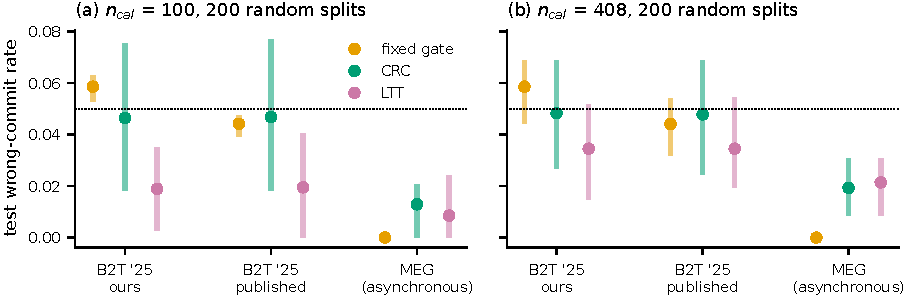
\includegraphics[width=\linewidth]{fig_crc_splits.pdf}
  \caption{\textbf{CRC bounds the mean over splits; LTT bounds the calibration-conditional risk with probability $1 - \delta$.} Test wrong-commit rate over 200 random calibration/test splits with (a)~100 and (b)~408 calibration items. Dots: mean; bars: 5th to 90th percentile (the 90th percentile matches $\delta = 0.1$). Dotted line: $\alpha = 0.05$. A test rate above $\alpha$ in a single split is not a violation of either guarantee.}
  \label{fig:crc}
\end{figure}
